\documentclass{beamer}
\usepackage{amsmath}
\usepackage{tikz}
\usepackage[utf8]{inputenc}
\usepackage{xcolor}

% Define custom colors
\definecolor{ds9blue}{RGB}{25,25,112}
\definecolor{ds9gold}{RGB}{218,165,32}
\definecolor{ds9grey}{RGB}{105,105,105}
\definecolor{ds9red}{RGB}{178,34,34}

% Theme setup
\usetheme{Madrid}
\usecolortheme{default}
\setbeamercolor{structure}{fg=ds9blue}
\setbeamercolor{title}{fg=ds9blue,bg=ds9gold!20}
\setbeamercolor{frametitle}{fg=ds9blue,bg=ds9gold!10}
\setbeamercolor{block title}{fg=white,bg=ds9blue}
\setbeamercolor{block body}{fg=black,bg=ds9gold!10}

% Title page setup
\title[Circular Motion]{PHYS11 CH6: Uniform Circular Motion}
\subtitle{Sections 6.1-6.4: Rotational Motion and Forces}
\author[Mr. Gullo]{Mr. Gullo}
\date[Feb 2025]{February, 2025}
\institute{Physics Department}

\begin{document}

\frame{\titlepage}

\begin{frame}
\frametitle{Learning Objectives}
\begin{block}{By the end of this presentation, you will be able to:}
\begin{itemize}
\item Define and calculate rotation angle and angular velocity
\item Explain centripetal acceleration and its properties
\item Analyze forces in circular motion
\item Understand non-inertial frames and fictitious forces
\end{itemize}
\end{block}
\end{frame}

\section{Rotational Motion}

\begin{frame}
\frametitle{Rotation Angle}
\begin{block}{Definition}
The rotation angle $\Delta\theta$ is defined as:
\[ \Delta\theta = \frac{\Delta s}{r} \]
where:
\begin{itemize}
\item $\Delta s$ = arc length
\item $r$ = radius of curvature
\end{itemize}
\end{block}
\begin{itemize}
\item Measured in radians (rad)
\item One complete revolution: $2\pi$ rad = 360°
\end{itemize}
\end{frame}

\begin{frame}
\begin{figure}
    \centering
    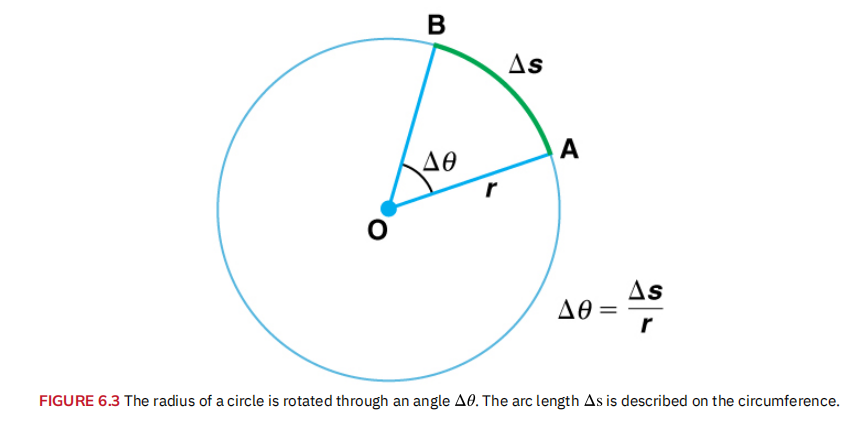
\includegraphics[width=1\linewidth]{CH6/arc.png}
\end{figure}
\end{frame}

\begin{frame}
\frametitle{Angular Velocity}
\begin{block}{Definition}
Angular velocity $\omega$ is the rate of change of angle:
\[ \omega = \frac{\Delta\theta}{\Delta t} \]
\end{block}
\begin{block}{Relationship to Linear Velocity}
\[ v = r\omega \]
where:
\begin{itemize}
\item $v$ = linear velocity
\item $r$ = radius
\item $\omega$ = angular velocity
\end{itemize}
\end{block}
\end{frame}

\begin{frame}
\begin{figure}
    \centering
    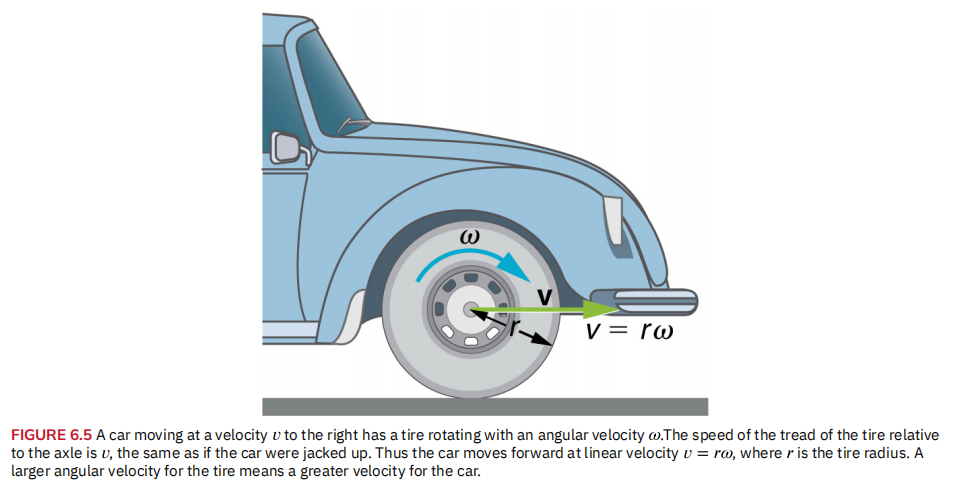
\includegraphics[width=1\linewidth]{CH6/wheelomega.png}
\end{figure}
\end{frame}

\section{Centripetal Acceleration}

\begin{frame}
\frametitle{Media}
     \begin{itemize}
  \item Centripetal Acceleration
  \item \hyperlink{https://www.youtube.com/watch?v=90rFibLktF4}{https://www.youtube.com/watch?v=90rFibLktF4}
  \item Application
  \item \hyperlink{https://youtu.be/im-JM0f_J7s?si=VO4FyEuT5SLf7Fzr}{https://youtu.be/im-JM0f_J7s?si=VO4FyEuT5SLf7Fzr}
  \end{itemize}
\end{frame}

\begin{frame}
\frametitle{Centripetal Acceleration}
\begin{block}{Definition}
Centripetal acceleration is the acceleration toward the center of circular motion:
\[ a_c = \frac{v^2}{r} = r\omega^2 \]
\end{block}
\begin{itemize}
\item Always points toward center of circle
\item Magnitude depends on speed and radius
\item Required for circular motion
\end{itemize}
\end{frame}

\begin{frame}
\begin{figure}
    \centering
    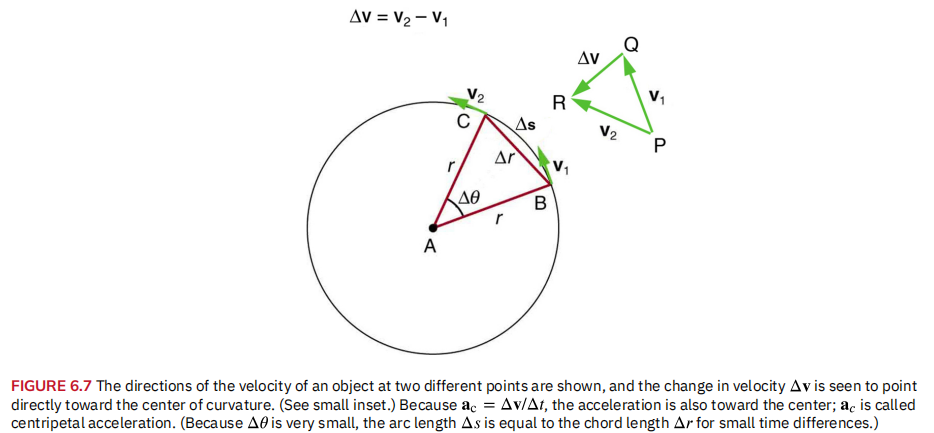
\includegraphics[width=1\linewidth]{CH6/centerseek.png}
\end{figure}
\end{frame}

\begin{frame}
\frametitle{Example: Centripetal Acceleration}
\begin{block}{I Do: Car on Curved Path}
A car travels around a curve of radius 100 m at 20 m/s.
Calculate the centripetal acceleration.
\end{block}
\begin{align*}
a_c &= \frac{v^2}{r} \\
&= \frac{(20\text{ m/s})^2}{100\text{ m}} \\
&= 4\text{ m/s}^2
\end{align*}
\end{frame}

\section{Centripetal Force}

\begin{frame}
\frametitle{Media}
     \begin{itemize}
  \item Centripetal Force
  \item \hyperlink{https://www.youtube.com/watch?v=4bMawIIWi7w}{https://www.youtube.com/watch?v=4bMawIIWi7w}
  \end{itemize}
\end{frame}
    

\begin{frame}
\frametitle{Centripetal Force}
\begin{block}{Definition}
The centripetal force required for circular motion is:
\[ F_c = ma_c = m\frac{v^2}{r} = mr\omega^2 \]
\end{block}
\begin{itemize}
\item Net force must point toward center
\item Can be provided by various forces:
  \begin{itemize}
  \item Tension
  \item Gravity
  \item Friction
  \item Normal force
  \end{itemize}
\end{itemize}
\end{frame}

\begin{frame}
\begin{figure}
    \centering
    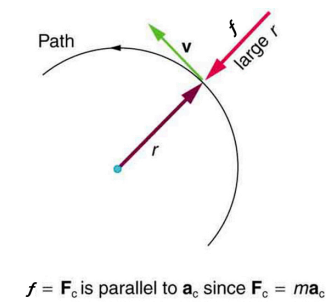
\includegraphics[width=1\linewidth]{CH6/centforce.png}
\end{figure}
\end{frame}

\begin{frame}
\frametitle{We Do: Centripetal Force Problem}
\begin{block}{Problem}
A 1000 kg car travels at 15 m/s around a curve of radius 50 m.
What centripetal force is required?
\end{block}
\begin{align*}
F_c &= m\frac{v^2}{r} \\
&= (1000\text{ kg})\frac{(15\text{ m/s})^2}{50\text{ m}} \\
&= 4500\text{ N}
\end{align*}
\end{frame}

\section{Non-inertial Frames}


\begin{frame}
\frametitle{Fictitious Forces}
\begin{block}{Key Points}
\begin{itemize}
\item Appear in non-inertial (accelerating) frames
\item Not "real" forces - arise from acceleration of reference frame
\item Examples:
  \begin{itemize}
  \item Centrifugal force
  \item Coriolis force
  \end{itemize}
\end{itemize}
\end{block}
\end{frame}
\begin{frame}
\frametitle{Media}
     \begin{itemize}
  \item Centrifugal force
  \item \hyperlink{https://www.youtube.com/watch?v=gRVIWWJwzfY}{https://www.youtube.com/watch?v=gRVIWWJwzfY}
  \end{itemize}
\end{frame}

\begin{frame}
\frametitle{Media}
     \begin{itemize}
  \item Coriolis force
  \item \hyperlink{https://www.youtube.com/watch?v=rdGtcZSFRLk}{https://www.youtube.com/watch?v=rdGtcZSFRLk}
  \end{itemize}
\end{frame}

\begin{frame}
\frametitle{The Coriolis Effect}
\begin{block}{Properties}
\begin{itemize}
\item Appears in rotating reference frames
\item Affects motion on rotating Earth
\item Causes deflection of:
  \begin{itemize}
  \item Weather systems
  \item Projectiles
  \item Ocean currents
  \end{itemize}
\end{itemize}
\end{block}
\end{frame}

\begin{frame}
\frametitle{You Do: Practice Problem}
\begin{block}{Problem}
A 0.5 kg ball is attached to a string and swung in a horizontal circle of radius 1.5 m.
If the ball makes one complete revolution in 2 seconds:
\begin{enumerate}
\item Calculate the angular velocity
\item Find the centripetal acceleration
\item Determine the tension in the string
\end{enumerate}
\end{block}
\end{frame}

\begin{frame}
\frametitle{Summary}
\begin{block}{Key Concepts}
\begin{itemize}
\item Angular quantities describe rotational motion
\item Centripetal acceleration points to center
\item Centripetal force causes circular motion
\item Fictitious forces appear in non-inertial frames
\end{itemize}
\end{block}
\end{frame}

\end{document}